\documentclass[11pt]{article}
\usepackage[utf8]{inputenc}
\usepackage[brazilian]{babel}

\usepackage{subfigure}
\usepackage[parfill]{parskip}
\usepackage{graphicx}
\usepackage[cm]{fullpage}
\usepackage{hyperref}
\usepackage{listings}
\lstset{
  basicstyle=\footnotesize\ttfamily,
}

\title{Compilando e Testando o Nanvix}

\author{Pedro H. Penna, Fernando Jorge Mota e Márcio Castro\\[0.3em]
\small Universidade Federal de Santa Catarina}
\date{}

\hyphenation{tool-chain}

\usepackage{url}

\begin{document}

\maketitle

%\begin{abstract}
\noindent 
%\end{abstract}


\section{Introdução}

Antes de começar a \textit{hackear} o Nanvix, é fundamental que você se familiarize com o modo como os arquivos do projeto estão organizados, com quais ferramentas de desenvolvimento você vai lidar e com o processo de compilação. Nesse primeiro projeto, você vai trabalhar em todas essas tarefas e, ao final, estará pronto para começar o trabalho duro.

É importante notar os scripts fornecidos para instalação e execução do Nanvix foram testados em distribuições Ubuntu e Lubuntu. Portanto, recomendamos fortemente que você utilize uma dessas duas distribuições. Certamente o Nanvix poderá ser compilado e executado em outras distribuições. Porém, será preciso em alguns casos realizar modificações nos scripts de instalação. 

Inicialmente mostraremos como baixar o código fonte do Nanvix e discutiremos sua estrutura de diretórios (Seção~\ref{sec:codigo}). Em seguida, mostraremos como instalar as ferramentas de desenvolvimento que permitirão a sua compilação (Seção~\ref{sec:ferramentas}). Posteriormente, mostraremos como compilar e executar o Nanvix (Seção~\ref{sec:compilacao}). Por fim, mostraremos uma forma alternativa de utilização do Nanvix através de uma Máquina Virtual (VM), permitindo assim que o sistema possa ser utilizado no Windows (Seção~\ref{sec:vm}). Da mesma forma, essa última solução permitirá o uso do Nanvix em sistemas Linux onde você não possui permissão de super-usuário.

\section{Código Fonte e Estrutura do Projeto}
\label{sec:codigo}
O primeiro passo para utilizar o Nanvix é baixar o seu código fonte. Para isso, basta clonar o seu repositório de desenvolvimento da seguinte forma\footnote{Caso você não tenha o \texttt{git} instalado, você poderá instalá-lo da seguinte forma: \texttt{sudo apt-get install git}}: \\

\begin{lstlisting}[language=bash,numbers=none,frame=single]
git clone https://github.com/ppenna/nanvix
\end{lstlisting}

Dentro do diretório do Nanvix você encontrará uma série de arquivos e diretórios. Por tratar-se de um projeto ligeiramente grande e complexo, o Nanvix é organizado em uma hierarquia de diretórios, que é detalhada a seguir:

\begin{itemize}
    \item \texttt{bin} conterá o binário do \textit{kernel} e utilitários, depois de terem sido compilados.
    \item \texttt{doc} contém toda a documentação do Nanvix, que inclui manuais do sistema, de bibliotecas e utilitários; orientações gerais para desenvolvimento; e documentação de APIs.
    \item \texttt{doxygen} contém arquivos de configuração da ferramenta Doxygen, que gera documentação das APIs do Nanvix diretamente do código fonte.
    \item \texttt{include} contém os arquivos-cabeçalhos de escopo global, tanto de sistema quanto de biblioteca.
    \item \texttt{lib} conterá todas as bibliotecas estáticas e dinâmicas, depois de terem sido compiladas.
    \item \texttt{src} contém o código fonte do Nanvix.
    \item \texttt{tools} contém todas as ferramentas e \textit{scripts} necessários para compilar o Nanvix.
\end{itemize}

\section{Instalação das Ferramentas e Ambiente de Desenvolvimento}
\label{sec:ferramentas}

As ferramentas utilizadas no desenvolvimento do Nanvix, como no desenvolvimento de qualquer outro sistema operacional, se diferem das utilizadas no desenvolvimento da maioria dos outros tipos de software. Em primeiro lugar, as ferramentas de compilação devem ser compatíveis com a plataforma alvo. Por exemplo, o Nanvix foi projetado para a plataforma x86, portanto as ferramentas utilizadas para compilar o sistema devem ser capazes de gerar código de máquina para essa plataforma. Em segundo lugar, quando trabalha-se em nível de \textit{kernel}, o ambiente de desenvolvimento não provê quaisquer tipo de bibliotecas padrões. Em terceiro lugar, para testar o sistema deve-se utilizar uma máquina dedicada, seja ela real ou virtual. Finalmente, em quarto lugar, as ferramentas de \textit{debugging} disponíveis são restritas.

Para o desenvolvimento do Nanvix, você utilizará duas ferramentas: a \textit{toolchain} GCC-x86, uma coletânea de utilitários que inclui compilador, \textit{assembler} e \textit{linker}; e o Bochs, um emulador para plataforma x86. Para instalar as ferramentas de forma automática execute os seguintes comandos \textbf{a partir do diretório raiz do projeto}: \\


\begin{lstlisting}[language=bash,numbers=none,frame=single]
sudo apt-get install make
sudo bash tools/dev/setup-toolchain.sh
sudo bash tools/dev/setup-bochs.sh
sudo reboot now
\end{lstlisting}

É esperado que o processo de instalação das ferramentas demore um certo tempo (vários minutos).

\section{Compilação e Execução}
\label{sec:compilacao}

Uma vez que as ferramentas de desenvolvimento necessárias para compilar o Nanvix foram devidamente instaladas, compilar o sistema torna-se uma tarefa simples. Do diretório raiz do projeto, invoque os seguintes comandos \textbf{a partir do diretório raiz do projeto}:\\

\begin{lstlisting}[language=bash,numbers=none,frame=single]
make nanvix
make image
\end{lstlisting}

O primeiro comando realiza a compilação do Nanvix. Terminado esse processo, todos os binários devem ter sido criados com sucesso. O segundo comando gera uma imagem do sistema, criando-se assim o arquivo \texttt{nanvix.img} no diretório raiz. Esse arquivo é a imagem do sistema e será usado no processo de \textit{boot}, a seguir.

Finalmente, inicie o Nanvix no Bochs, dando \textit{boot} pela imagem de sistema gerada. Para fazer isso de forma automática, execute o seguinte comando \textbf{a partir do diretório raiz do projeto}:\\

\begin{lstlisting}[language=bash,numbers=none,frame=single]
bash tools/run/run.sh
\end{lstlisting}

Pronto! Em caso de sucesso, você verá o Nanvix sendo inicializado. Após a inicialização, a tela principal do terminal do Nanvix está pronta para utilização, conforme mostra a Figura~\ref{fig:terminal-nanvix}.

\begin{figure}[t]
	\centering
	\subfigure[Nanvix.]{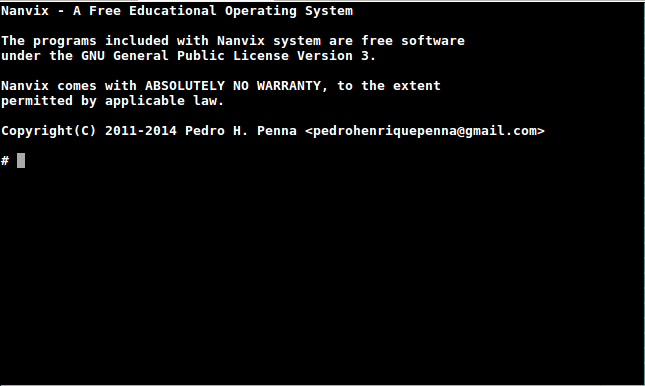
\includegraphics[scale=0.32]{img/terminal-nanvix.png}\label{fig:terminal-nanvix}}
	\qquad
	\subfigure[GDB.]{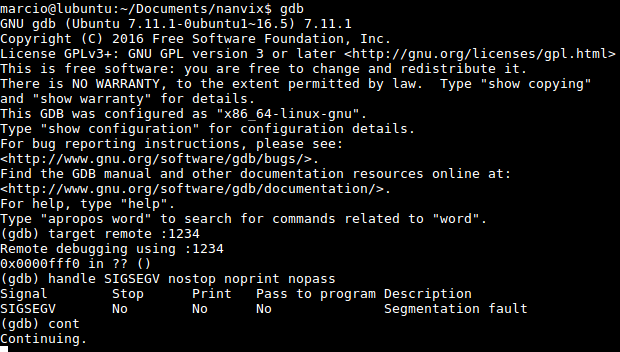
\includegraphics[scale=0.35]{img/terminal-GDB.png}\label{fig:terminal-gdb}}
\caption{Terminais do Nanvix e do GDB.}
\end{figure}

\section{\textit{Debugging} com o Nanvix}

Para realizar o \textit{debug} do Nanvix, o que pode ser muito útil na resolução de \textit{bugs} e outros problemas que surgirão durante o desenvolvimento de código no \textit{kernel}, será necessário o uso do \textit{gdb}, cujo uso e integração serão definidos nessa seção.

Para começar, utilize o seguinte comando para inicializar o Bochs com suporte ao GDB em um terminal: \\

\begin{lstlisting}[language=bash,numbers=none,frame=single]
bash tools/run/run.sh --debug
\end{lstlisting}

\textbf{Observação Importante}: Caso você esteja numa conexão remota (ex.: ssh), é extremamente sugerido o uso do \texttt{tmux} para evitar a necessidade de criar mais de uma conexão \textit{ssh}, visto que quando o \textit{bochs} está rodando ele assume o comando do shell inteiro. Neses caso, instale o tmux, usando \texttt{sudo apt-get install tmux}, execute o comando \texttt{tmux}, e pressione CTRL+B+\% para abrir dois \textit{panes}. Em seguida, use CTRL+B+(seta para direita ou seta para a esquerda) para alterar livremente pelos terminais. Mais informações podem ser vistas diretamente no manual do \texttt{tmux}: \url{https://leanpub.com/the-tao-of-tmux/read}


Depois, inicialize o GDB \textbf{em um outro terminal} a partir do diretório raiz do projeto, usando o seguinte comando: \\

\begin{lstlisting}[language=bash,numbers=none,frame=single]
gdb
\end{lstlisting}

E, então, no \textit{shell} do GDB, execute os seguintes comandos:\\

\begin{lstlisting}[language=sh,numbers=none,frame=single]
target remote :1234
handle SIGSEGV nostop noprint nopass
cont
\end{lstlisting}

Segue uma explicação breve aos comandos informados acima:

\begin{enumerate}
	\item Conecta-se ao \textit{Bochs}, que agora mostrará que há um cliente conectado;
	\item Define que \textit{page faults} e outras interrupções frequentes devem ser ignoradas completamente pelo GDB. O \texttt{SIGSEGV} aqui é apenas um \textit{alias} para representar essas outras interrupções que são normais durante a execução da máquina;
	\item Define que a máquina deve continuar sua execução. Depois de realizar esse comando o \textit{shell} do Nanvix ficará disponível na tela do \textit{Bochs}.
\end{enumerate}

Pronto! Em caso de sucesso você verá o GDB conectado ao Bochs, como mostra a Figura~\ref{fig:terminal-gdb}. Para realizar o \textit{debug} do \textit{kernel}, você pode usar o comando:\\

\begin{lstlisting}[language=sh,numbers=none,frame=single]
symbol-file bin/kernel
\end{lstlisting}

Observe que, se o objetivo aqui for realizar o \textit{debug} de algum programa dentro do Nanvix (como o \texttt{ls}, por exemplo), é necessário executar o mesmo comando mas informando o caminho executável dentro da pasta \texttt{bin}, por exemplo:\\

\begin{lstlisting}[language=sh,numbers=none,frame=single]
symbol-file bin/ubin/ls
\end{lstlisting}

Observe que não é recomendável usar mais de uma tabela de símbolos ao mesmo tempo, pois nesse caso o GDB não é capaz de diferenciar corretamente a respeito do quê está ocorrendo no sistema. Logo, ao realizar esse comando em um \textit{shell} onde a tabela de símbolos do \textit{kernel} já foi carregada o GDB perguntará se a tabela de símbolos deve ser substituída, o que é necessário para realizar o \textit{debugging} de um programa do Nanvix.

Para definir \textit{breakpoints}, você pode usar o comando \texttt{b} \textbf{depois da tabela de símbolos ser carregada}. Para fazer um \textit{debug} da função \texttt{yield}, por exemplo, é possível simplesmente fazer:\\

\begin{lstlisting}[language=sh,numbers=none,frame=single]
b yield
\end{lstlisting}

No lugar do nome da função, você pode também definir uma linha onde o GDB deve definir o \textit{breakpoint}. Dessa forma, você pode usar o seguinte comando para definir um \textit{breakpoint} na linha 143 do arquivo \textbf{main.c}, por exemplo:\\

\begin{lstlisting}[language=sh,numbers=none,frame=single]
b main.c:143
\end{lstlisting}

Observe que a função de \textit{breakpoint} só funciona bem se você carregar a tabela de símbolos usando o comando \textit{symbol-file}, anteriormente especificado, pois é a partir da tabela de símbolos que o GDB consegue identificar os arquivos e funções envolvidos.

A partir do \textit{breakpoint}, é possível usar o comando \texttt{step} para saltar para a próxima instrução:\\

\begin{lstlisting}[language=sh,numbers=none,frame=single]
step
\end{lstlisting}

Você também pode saltar um número definido de instruções com uso de um parâmetro opcional do \texttt{step}. Por exemplo, utilize o seguinte comando para saltar 10 instruções de uma única vez:\\

\begin{lstlisting}[language=sh,numbers=none,frame=single]
step 10
\end{lstlisting}

O comando \texttt{step} permite realizar um \textit{bug} do tipo \textit{step by step}. Isso significa que quando uma função é executada durante o \textit{debug}, o \textit{bugger} fará o desvio para a primeira instrução da função. Caso você queira saltar diretamente para o retorno da função, você poderá utilizar o comando \texttt{next}:\\

\begin{lstlisting}[language=sh,numbers=none,frame=single]
next
\end{lstlisting}

Por fim, para simplesmente pular toda a execução você pode usar o comando \texttt{cont} (que fará com que o \textit{GDB} só pare a execução no próximo \textit{breakpoint}): \\

\begin{lstlisting}[language=sh,numbers=none,frame=single]
cont
\end{lstlisting}

Além disso, durante o \textit{debug}, é interessante usar o comando \texttt{print} para imprimir variáveis que possam ser úteis para entender a execução do código. Dessa forma, para imprimir a variável global \texttt{curr\_proc}, que está presente no \textit{kernel} do Nanvix, é possível usar:\\

\begin{lstlisting}[language=sh,numbers=none,frame=single]
print curr_proc
\end{lstlisting}

Da mesma forma, é possível usar parte da sintaxe do C para explorar os diferentes atributos que a variável possa ter. Por exemplo:\\

\begin{lstlisting}[language=sh,numbers=none,frame=single]
print curr_proc->pid
\end{lstlisting}

O comando acima imprime o PID do processo atual em execução (no caso do Nanvix, o PID é um atributo de \texttt{curr\_proc}). Observe que o \texttt{print} também funciona em \textit{breakpoints}, com variáveis locais, sendo portanto bastante útil para entender o que está acontecendo no código.

Por fim, para saber a sequência de chamadas atual, você pode usar o comando \textit{bt}, que imprime o \textit{back-trace} atual do código.

\textbf{Observação importante:} O Bochs não suporta determinadas operações que o GDB suporta, como \texttt{watch} (para acompanhar o valor de uma variável ao longo do tempo), ou chamadas de função no \texttt{print}. Fazer isso resulta ou em erro, ou em instabilidade do sistema, ou nos dois. Portanto, sua realização não é recomendada. 

Para mais informações a respeito do GDB, consulte o manual em: \url{https://sourceware.org/gdb/current/onlinedocs/gdb/}

\section{Nanvix no Windows em uma Máquina Virtual (VM)}
\label{sec:vm}

Caso você não tenha uma máquina com Linux e não tenha interesse em instalá-lo diretamente na sua máquina\footnote{Que triste... Deveria ter!}, você poderá fazer uma instalação do Linux em uma Máquina Virtual (VM) rodando no Windows. Nesse caso, aconselhamos a utilização do \textit{Virtual Box}
(disponível em \url{www.virtualbox.org}). Após instalar o Virtual Box, aconselhamos a instalação do Lubuntu 16.04 (disponível em \url{http://lubuntu.net}) na VM, pois trata-se de uma distribuição relativamente leve e testada. Por fim, basta seguir os passos de instalação e compilação (Seções~\ref{sec:codigo} a~\ref{sec:compilacao}) do Nanvix no Lubuntu.

\end{document}
